\documentclass[a4paper, 12pt]{article}
\usepackage[utf8x]{inputenc}
\usepackage[english, russian]{babel}
\usepackage[left=25mm, top=25mm, right=25mm, bottom=25mm]{geometry}
\usepackage{cmap}
\usepackage{indentfirst}
\usepackage{tikz}
\usepackage{float}
\usepackage{amsmath, amsfonts, amssymb}
\usepackage{graphicx}
\usepackage{hyperref}
\usepackage{listings}
\usepackage{caption}
\usepackage{subcaption}
\usepackage{xcolor}
\usepackage{etoolbox}
\usepackage{titlesec}
\pagestyle{plain}
\patchcmd{\tableofcontents}{\contentsname}{\centering\contentsname}{}{}
\titleformat{\section}[block]{\normalfont\large\bfseries\centering}{}{0pt}{}
\titleformat{\subsection}[block]{\normalfont\normalsize\bfseries\centering}{}{0pt}{}
\allowdisplaybreaks
\graphicspath{{images/}}
\usetikzlibrary{patterns}
\definecolor{LightGray}{gray}{0.95}
\definecolor{LightGray2}{gray}{0.7}
\lstdefinestyle{code}{
    language=MATLAB, % replace language here
    basicstyle=\footnotesize\ttfamily,
    % numbers=left,
    % numberstyle=\scriptsize\color{gray},
    % stepnumber=1,
    % numbersep=5pt,
    backgroundcolor=\color{LightGray},
    showspaces=false,
    showstringspaces=false,
    showtabs=false,
    tabsize=4,
    captionpos=b,
    breaklines=true,
    breakatwhitespace=false,
    frame=single,
    rulecolor=\color{LightGray2},
    linewidth=\linewidth,
    keywordstyle=\color{blue}\bfseries,
    commentstyle=\color{green!40!black},
    stringstyle=\color{purple},
    escapeinside={\%*}{*)},
    inputencoding=utf8x,
    xleftmargin=0pt,
    framexleftmargin=0pt,
    framexrightmargin=0pt
}
\lstset{style=code}
\hypersetup{
    colorlinks=true,
    linkcolor=blue,
    filecolor=magenta,
    urlcolor=cyan,
    pdftitle={contents setup},
    pdfpagemode=FullScreen,
}


\begin{document}
    \begin{titlepage}

        \begin{center}
        Федеральное государственное автономное образовательное учреждение высшего образования
        «Национальный Исследовательский Университет ИТМО»
        \vfill
        
        
\includegraphics[width=0.3\textwidth]{itmo.png} % requires /images/itmo.png

        {\large\bf ЛАБОРАТОРНАЯ РАБОТА №1}\\
        {\large\bf ПРЕДМЕТ «ТЕОРИЯ АВТОМАТИЧЕСКОГО УПРАВЛЕНИЯ»}\\
        {\large\bf ТЕМА «УПРАВЛЯЕМОСТЬ И НАБЛЮДАЕМОСТЬ»}
        Вариант №2
        \vfill

        \begin{flushright}
            \begin{minipage}{.45\textwidth}
            {
                \hbox{Преподаватель:}
                \hbox{Пашенко А. В.}
                \hbox{}
                \hbox{Выполнил:}
                \hbox{Румянцев А. А.}
                \hbox{}
                \hbox{Факультет: СУиР}
                \hbox{Группа: R3341}
                \hbox{Поток: ТАУ R22 бак 1.1.1}
            }
            \end{minipage}
        \end{flushright}
        \vfill
  
        Санкт-Петербург\\
        2025
        \end{center}
    \end{titlepage}
    
    \tableofcontents

    \newpage
    \section{Задание 1. Исследование управляемости}
    Рассмотрим систему $$\dot{x}=Ax+Bu,\text{ где } A=\begin{bmatrix}
        1 &-2 &3\\
        2 &-3 &2\\
        -2 &1 &-4
    \end{bmatrix},\ B=\begin{bmatrix}
        -3\\
        -1\\
        3
    \end{bmatrix};\text{ дана точка } x_1=\begin{bmatrix}
        4\\
        3\\
        -3
    \end{bmatrix}$$


    \subsection{Матрица управляемости}
    Исходя из условия видим, что порядок системы $n$ равен трем. Значит, матрица управляемости будет иметь вид
    $$U=\begin{bmatrix}
        B &AB &A^2B
    \end{bmatrix}$$
    Вектор $B$ нам известен. Найдем оставшиеся неизвестные
    $$AB=\begin{bmatrix}
        1 &-2 &3\\
        2 &-3 &2\\
        -2 &1 &-4
    \end{bmatrix}\begin{bmatrix}
        -3\\
        -1\\
        3
    \end{bmatrix}=\begin{bmatrix}
        8\\
        3\\
        -7
    \end{bmatrix},$$
    $$A^2B=\begin{bmatrix}
        1 &-2 &3\\
        2 &-3 &2\\
        -2 &1 &-4
    \end{bmatrix}^2\begin{bmatrix}
        -3\\
        -1\\
        3
    \end{bmatrix}=\begin{bmatrix}
    -9	 &7	&-13\\
    -8	 &7	 &-8\\
    8	&-3	 &12
    \end{bmatrix}\begin{bmatrix}
        -3\\
        -1\\
        3
    \end{bmatrix}=\begin{bmatrix}  
    -19\\
    -7\\
    15
    \end{bmatrix}$$
    Таким образом, получаем матрицу управляемости
    $$
    U=\begin{bmatrix}
        -3 &8 &-19\\
        -1 &3 &-7\\
        3 &-7 &15
    \end{bmatrix}
    $$
    Определим ранг этой матрицы, чтобы сделать вывод об управляемости системы в целом
    $$
    \text{rank}\left[U\right]=\text{rank}\begin{bmatrix}
        -3 &8 &-19\\
        -1 &3 &-7\\
        3 &-7 &15
    \end{bmatrix}=3
    $$
    Так как ранг матрицы управляемости равен порядку системы $n$, то система является полностью управляемой


    \subsection{Собственные числа и матрицы Хаутуса}
    Найдем собственные числа матрицы $A$
    $$\det\left[\lambda I -A\right]=\begin{vmatrix}
        \lambda-1 &2 &-3\\
        -2 &\lambda+3 &-2\\
        2 &-1 &\lambda+4
    \end{vmatrix}=\lambda^3+6\lambda^2+13\lambda+10=0$$
    Подбором получаем корень $\lambda_1=-2$. Вынесем его за скобку, и, решим квадратное уравнение
    $$\left(\lambda+2\right)\left(\lambda^2+4\lambda+5\right)=0,$$
    $$\lambda^2+4\lambda+5=0,\ D=4^2-5\cdot4=-4\Rightarrow\lambda_{2,3}=\dfrac{-4\pm2i}{2}=-2\pm i$$
    Таким образом, матрица $A$ имеет следующие собственные числа
    \begin{align*}
        &\lambda_1=-2\\
        &\lambda_{2,3}=-2\pm i
    \end{align*}
    Действительная часть всех собственных чисел меньше нуля, а значит они все асимптотически устойчивые, но могут быть неуправляемыми.
    Для проверки построим матрицы Хаутуса $\left[A-\lambda_i I\ B\right]$ для каждого собственного числа и найдем их ранг
    $$\text{rank}\left[A-\lambda_1 I\ B\right]=\text{rank}\begin{bmatrix}
        3 &-2 &3 &-3\\
        2 &-1 &2 &-1\\
        -2 &1 &-2 &3
    \end{bmatrix}=3$$
    $$\text{rank}\left[A-\lambda_{2,3} I\ B\right]=\text{rank}\begin{bmatrix}
        3\pm i &-2 &3 &-3\\
        2 &-1\pm i &2 &-1\\
        -2 &1 &-2\pm i &3
    \end{bmatrix}=3$$
    Ранги матриц Хаутуса для каждого собственного числа матрицы $A$ равны порядку системы, следовательно, все
    собственные числа являются управляемыми. Из этого же следует, что система полностью управляема


    \subsection{Жорданова форма системы}
    Мы можем разложить матрицу $A$ следующим образом
    $$A=PJP^{-1},$$ где $P$ -- матрица собственных векторов матрицы $A$, $J$ -- жорданова нормальная форма.
    В нашем случае кратных собственных чисел нет, а значит ЖНФ примет вид диагональной матрицы. Это объясняется тем,
    что для каждого собственного числа найдется хотя бы один собственный вектор ($A\textbf{v}=\lambda\textbf{v}$),
    то есть каждому собственному числу соответствует ровно одна жорданова клетка размера $1\times1$. Ранее мы
    вычисляли собственные числа -- составим матрицу $J$ без поиска $P$ и $P^{-1}$
    $$J=\begin{bmatrix}
        \lambda_1 &0 &0\\
        0 &\lambda_2 &0\\
        0 &0 &\lambda_3
    \end{bmatrix}=
    \begin{bmatrix}
        -2 &0 &0\\
        0 &-2-i &0\\
        0 &0 &-2+i
    \end{bmatrix}$$
    Более того, можно сделать матрицу вещественной, пользуясь знаниями с линейной алгебры
    $$
    \lambda_{1,2}=\alpha\pm\beta i,\ J=\begin{bmatrix}
        \alpha+\beta i &0\\
        0 &\alpha-\beta i
    \end{bmatrix}\Rightarrow J_{re}=\begin{bmatrix}
        \alpha &\beta\\
        -\beta &\alpha
    \end{bmatrix}
    $$
    Получаем матрицу $J_{re}$ в базисе собственных векторов матрицы $A$
    $$
    J_{re}=\begin{bmatrix}
        -2 &0 &0\\
        0 &-2 &1\\
        0 &-1 &-2
    \end{bmatrix}=P_{re}^{-1}AP_{re}
    $$
    Далее для анализа необходимо перевести вектор входных воздействий $B$ в базис собственных векторов матрицы $A$
    $$B_{Jre}=P_{re}^{-1}B$$
    Для поиска $P_{re}$ составим матрицу собственных векторов $P$ матрицы $A$
    ($v_i$ находятся подстановкой соответсвующих $\lambda_i$ в $\left[\lambda_i I-A\right]$ и решением СЛАУ)
    $$P=\left[v_1\ v_2\ v_3\right]=\begin{bmatrix}
        -1 &-1.5+0.5i &-1.5-0.5i\\
        0 &-1 &-1\\
        1 &1 &1
    \end{bmatrix}$$
    Теперь составим матрицу $P_{re}$ по следующему принципу: каждый нечетный столбец составляется из действительных
    частей чисел соответствующих нечетных столбцов матрицы $P$, а каждый четный -- из мнимых частей
    $$P_{re}=\left[\Re{\left\{P_1\right\}}\ \Im{\left\{P_2\right\}}\ \Re{\left\{P_3\right\}}\right]=\begin{bmatrix}
        -1 &0.5 &-1.5\\
        0 &0 &-1\\
        1 &0 &1
    \end{bmatrix}$$
    Найдем обратную матрицу от $P_{re}$ и вычислим $B_{Jre}$
    $$
    P_{re}^{-1}=\begin{bmatrix}
        -1 &0.5 &-1.5\\
        0 &0 &-1\\
        1 &0 &1
    \end{bmatrix}^{-1}=\begin{bmatrix}
        0 &1 &1\\
        2 &-1 &2\\
        0 &-1 &0
    \end{bmatrix}\Rightarrow
    P_{re}^{-1}B=\begin{bmatrix}
        0 &1 &1\\
        2 &-1 &2\\
        0 &-1 &0
    \end{bmatrix}\begin{bmatrix}
        -3\\
        -1\\
        3
    \end{bmatrix}=\begin{bmatrix}
        2\\
        1\\
        1
    \end{bmatrix}=B_{Jre}
    $$
    Мы так же можем убедиться, что верно нашли $J_{re}$
    $$J_{re}=P_{re}^{-1}AP_{re}=\begin{bmatrix}
        0 &1 &1\\
        2 &-1 &2\\
        0 &-1 &0
    \end{bmatrix}\begin{bmatrix}
        1 &-2 &3\\
        2 &-3 &2\\
        -2 &1 &-4
    \end{bmatrix}\begin{bmatrix}
        -1 &0.5 &-1.5\\
        0 &0 &-1\\
        1 &0 &1
    \end{bmatrix}=\begin{bmatrix}
        -2 &0 &0\\
        0 &-2 &1\\
        0 &-1 &-2
    \end{bmatrix}$$
    Итого, получаем
    $$
    J_{re}=\begin{bmatrix}
        -2 &0 &0\\
        0 &-2 &1\\
        0 &-1 &-2
    \end{bmatrix},\
    B_{Jre}=\begin{bmatrix}
        2\\
        1\\
        1
    \end{bmatrix}
    $$
    Мы уже выяснили, что все жордановы клетки относятся к различным собственным числам -- можем делать выводы об управляемости.
    Так как элементы матрицы входных воздествий $B_{Jre}$ не равны нулю, то все собственные числа управляемы. Из этого следует, что
    система полностью управляема. При этом достаточное условие полной управляемости системы в нашем случае -- не равенство нулю
    последнего элемента матрицы $B_{Jre}$.


    \subsection{Грамиан управляемости системы}
    Найдем Грамиан управляемости системы относительно времени $t_1=3$
    $$P(t_1)=\int\limits_{0}^{t_1}e^{At}BB^Te^{A^Tt}\,dt$$
    Предоставим вычисления \texttt{MATLAB}. Программа представлена на листинге \ref{task1} в приложении 1. Итого имеем
    $$P(t_1=3)=\begin{bmatrix}
    1.5956    &0.4779   &-1.7132\\
    0.4779    &0.1500   &-0.5029\\
   -1.7132   &-0.5029    &1.8559
    \end{bmatrix}$$
    Получили числовую матрицу. Для анализа управляемости системы найдем собственные числа Грамиана с помощью \texttt{MATLAB}. Получаем
    \begin{align*}
    \lambda_1=3.5841\\
    \lambda_2=0.0002\\
    \lambda_3=0.0172
    \end{align*}
    Все собственные числа Грамиана относительно $t_1=3$ строго положительны, следовательно, его определитель (произведение собственных чисел) больше нуля -- Грамиан невырожденный.
    Это следует уже из равенства ранга матрицы управляемости порядку системы -- полученный в нынешнем пункте результат подтверждает наши рассуждения -- система полностью управляема.
    Однако из-за присутствия маленького собственного числа $\lambda_2=0.0002$ можно сделать вывод, что в некотором направлении система слабо управляема.


    \subsection{Управление системой за определенное время}
    Найдем управление, переводящее систему из $x(0)=0$ в $x(t_1)=x_1$ за время $t_1$, по формуле
    $$u(t)=B^Te^{A^T(t_1-t)}\left[P(t_1)\right]^{-1}x_1$$
    Подставим матрицы и $t_1$ в выражение
    $$u(t)=\begin{bmatrix}
        -3\\
        -1\\
        3
    \end{bmatrix}^T
    e^{\begin{bmatrix}
        1 &-2 &3\\
        2 &-3 &2\\
        -2 &1 &-4
    \end{bmatrix}^T\left(3-t\right)}\begin{bmatrix}
        1.5956    &0.4779   &-1.7132\\
        0.4779    &0.1500   &-0.5029\\
       -1.7132   &-0.5029    &1.8559
    \end{bmatrix}^{-1}\begin{bmatrix}
        4\\
        3\\
        -3
    \end{bmatrix}$$
    После всех вычислений получим
    $$
    u(t)=\dfrac{17826740000e^{2t}-17213830000e^2\cos{(3-t)}-6911070000e^2\sin{(3-t)}}{13222909e^6}    
    $$
    Мы нашли управление, переводящее систему из $x(0)=0$ в $x(t_1)=x_1$ за время $t_1$. Выполним моделирование системы
    в \texttt{MATLAB}. Зададим интервал $t\in\left[0,t_1=3\right]$ с 1000 точками.
    Для каждого $t_i$ вычислим по формуле $u_i(t_i)$, после чего построим график $u(t)$. Для моделирования изменения состояния
    системы во времени решим СДУ $\dot{x}=Ax+Bu(t)$ с начальным условием $x(0)=0$, после чего построим график
    \begin{figure}[H]
        \centering
        \begin{subfigure}{0.45\textwidth}
            \centering
            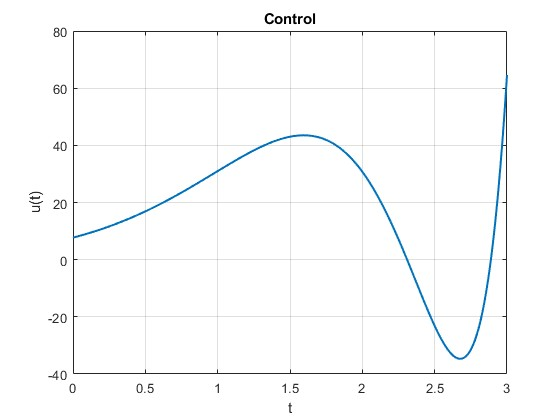
\includegraphics[width=\linewidth]{task_1_u_t.jpg}
            \caption{График $u(t)$}
            \label{fig:task_1_u_t}
        \end{subfigure}
        \hfill
        \begin{subfigure}{0.45\textwidth}
            \centering
            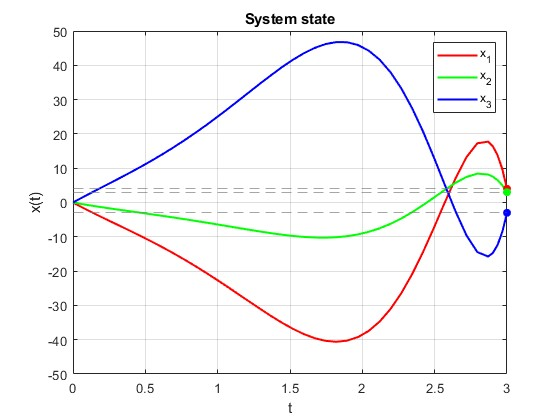
\includegraphics[width=\linewidth]{task_1_x_t.jpg}
            \caption{График $x(t)$}
            \label{fig:task_1_x_t}
        \end{subfigure}
        \caption{Графики для первого задания}
        \label{fig:task_1_modeling}
    \end{figure}
    \noindent Серыми пунктирными линиями на графике $x(t)$ отмечены координаты вектора $x_1=\left[4\ 3\ -3\right]^T$.
    Как видим, система достигает состояния $x_1$ в момент времени $t_1=3$ -- $x_i$ сходятся к соответствующим пунктирным линиям


    \subsection{Выводы}
    Все собственные числа матрицы $A$ управляемы, система полностью управляема. Моделирование системы подтвердило наши рассуждения.


    \section{Задание 2. Еще одно исследование управляемости}


    \section{Приложения}
    \subsection{Приложение 1}
    \begin{lstlisting}[label=task1, caption={Программа для первого задания}]
    % input data
    A = [1 -2 3; 2 -3 2; -2 1 -4];
    B = [-3; -1; 3];
    x1 = [4; 3; -3];
    t1 = 3;

    % controllability matrix
    U = [B A*B A*A*B];
    r = rank(U);
    disp(U);
    disp(r);

    % A matrix eigenvalues
    A_e = eig(A);
    disp(A_e);

    % Houtus matrices
    H_1 = [A-A_e(1)*eye(3) B];
    r_1 = rank(H_1);
    disp(H_1);
    disp(r_1);

    H_2 = [A-A_e(2)*eye(3) B];
    r_2 = rank(H_2);
    disp(H_2);
    disp(r_2);

    H_3 = [A-A_e(3)*eye(3) B];
    r_3 = rank(H_3);
    disp(H_3);
    disp(r_3);

    % Jordan matrix
    [P, J] = jordan(A);
    P1(:,1) = real(P(:,1));
    P1(:,2) = imag(P(:,2));
    P1(:,3) = real(P(:,3));
    P1_inv = P1^-1; 
    J_re = P1_inv * A * P1;
    B_jre = P1_inv * B;
    disp(P1);
    disp(P1_inv);
    disp(J_re);
    disp(B_jre);

    % gramian
    integrand = @(t) expm(A * t) * (B * B') * expm(A' * t);
    P_t1 = integral(@(t) integrand(t), 0, t1, 'ArrayValued', true);
    disp(P_t1);

    % gramian eigenvalues
    e = eig(P_t1);
    disp(e);

    % u_t
    u_t = @(t) B' * expm(A' * (t1 - t)) * inv(P_t1) * x1;

    % u_t modeling
    time = linspace(0, t1, 1000);

    control = arrayfun(@(t) u_t(t), time, 'UniformOutput', false);
    control = cell2mat(control);

    figure;
    plot(time, control, 'LineWidth', 1.5);
    xlabel('t');
    ylabel('u(t)');
    title('Control');
    grid on;

    % x_t
    dxdt = @(t, x) A * x + B * u_t(t);

    % x_t modeling
    [t, x] = ode45(dxdt, [0 t1], [0; 0; 0]);

    figure;
    plot(t, x, 'LineWidth', 1.5);
    yline(x1(1), '--', 'Color', [0.5 0.5 0.5]); % x_1
    yline(x1(2), '--', 'Color', [0.5 0.5 0.5]); % x_2
    yline(x1(3), '--', 'Color', [0.5 0.5 0.5]); % x_3
    xlabel('t');
    ylabel('x(t)');
    legend('x_1', 'x_2', 'x_3');
    title('System state');
    grid on;
    \end{lstlisting}
\end{document}